\documentclass{article}
\usepackage[utf8]{inputenc}
\usepackage{natbib}
\usepackage{graphicx}
\usepackage{amsmath}
\usepackage{array}

%----------------------------------------------------------------

\begin{document}

\begin{titlepage}

\vspace*{\fill} 
\begin{center} 
    \hline
     \vspace{5mm}
    \Huge{\bfseries Protracktor\\Local Proctoring and Activity Tracker}\\
     \vspace{5mm}
    \hline
    \vspace{10mm}
    \LARGE{\textbf{Quad-Core}}\\
    \vspace{5mm}
    \begin{tabular}{c c}
    Amit Kumar Bala Antu & 203051003\\
    Kunal Verma & 203050121\\
    Mallela Niteesh Kumar Reddy & 203050065\\
    Nimesh Aggarwal & 203050049\\
    Shubhranshu Maurya & 203050096\\
    \end{tabular}
    %[2mm]

\end{center}
\vspace*{\fill}
\end{titlepage}

%\newpage
\tableofcontents
\newpage

%----------------------------------------------------------------

\section{Introduction}

\subsection{Motivation}
Today due to the COVID-19 pandemic schools, colleges and students are facing an unprecedented situation which has led to online learning and conducting of proctored examinations through video conferencing a new normal.\\
This new pattern of learning and conducting exams has created several challenges for both students as well as teachers. Students are facing several issues related to prolonged screen time, network & data related issues while attempting a proctored quiz, procrastination and sometimes inadvertently spending too much time on screen on certain unproductive activities.\\
We came up with an idea of \textbf{Protracktor} which will try to tackle the above issues to make this system more streamlined for students.


\subsection{Objective}
Through Protracktor our objective was to develop such an application which:
\begin{itemize}
    \item Keeps track of network connectivity and also tries to maintain a report of data consumption by each process in use. This could help one to plan their daily data consumption by each application.
    \item Keeps track of your screen time - the current application in use - to give a better understanding of how much time on each process one is spending. This will help one to manage their screen time accordingly.
    \item During online proctored tests and quizzes students face network connectivity issues where if a student loses internet connectivity then they have to turn on the camera and screen recorder. While attempting the tests it creates too much hassle and distraction we also wish to automate this process and incorporate it in the application such that as soon the internet goes off it will start the recording.
\end{itemize}

%----------------------------------------------------------------

\section{Dependencies}
\begin{itemize}
    \item Python3
    \item OpenCV
    \item xdotools
    \item nethogs
    \item urllib
    \item Tkinter
    \item PyQt5
    \item PyAutoGUI
    \item time
    \item Threading
    \item subprocess
    \item matplotlib
    \item operator
    \item json
    \item notify2
    \item signal
    \item CSV
\end{itemize}

%----------------------------------------------------------------

\section{Using Protracktor}
The initial build support only linux based platforms.
\subsection{Getting dependencies ready}
In order to use Protracktor you first need to make sure you have all the dependencies installed. If you haven't installed them don't worry we have your back.\\
We have made an installer.sh file which will take care of all the dependencies and requirements for the project.\\
To run installer.sh, go to the project directory "Protracktor$>$source" where installer.sh is present and then run the following commands\\
\begin{verbatim}
    $ chmod +x installer.sh
    $ ./installer.sh
\end{verbatim}

If some requirements are still missed please follow the steps below to manually install the dependencies.\\
Install python on your system by running the following command on your terminal:
\begin{verbatim}
    $ sudo apt-get install python3.6
\end{verbatim}
Screen activity module needs \verb|xdotool| to get window's information.
\begin{verbatim}
    $ sudo apt-get install xdotool
\end{verbatim}
For Internet Tracking Module install \verb|nethogs| 
\begin{verbatim}
    $ sudo apt-get install nethogs
    $ sudo setcap "cap_net_admin,cap_net_raw=ep" /usr/sbin/nethogs
\end{verbatim}
To install \verb|PyAutoGUI| additionally you need to install the \verb|scrot| application, as well as Tkinter and other python libraries requirement: 
\begin{verbatim}
    $ sudo apt-get install scrot
    $ sudo apt-get install python3-tk
    $ sudo apt-get install python3-dev
    $ sudo pip3 install pyautogui
    $ sudo pip3 install python3-xlib
    $ sudo pip3 install numpy==1.18.5
    $ sudo pip3 install notify2==0.3.1
    $ sudo pip3 install matplotlib==3.3.1
    $ sudo pip3 install opencv_python==4.1.2.30
    $ sudo pip3 install PyQt5==5.15.1
\end{verbatim}




All the functionalities and how to use them is depicted ahead in the next section.

\section{How To-Guide}

%----------------------------------------------------------------
After installing all the dependencies and the requirements only thing left is see how to operate our program.\\
Go to the main directory "Protracktor" and in that go to source directory. After that run the following command in terminal
\begin{verbatim}
    $ python3 main.py
\end{verbatim}
This will start the application!
\subsection{Main window}
The main window has two tabs namely "Local Proctoring" and "Let's Start"\\
\begin{center}
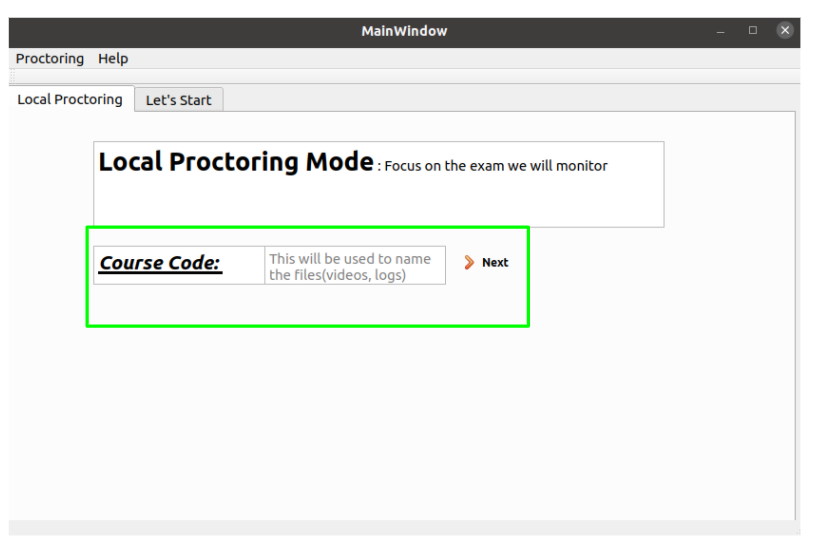
\includegraphics[scale=0.8]{MainWindow.png}    
\end{center}

\begin{enumerate}
    \item First enter the course code you want to start proctoring for.
    \item This field is used to name the log files and video files with additional timestamps added as a naming convention for files
    \item Click on "Next" to move to the next tab "Let's Start"
    
\end{enumerate}
On clicking next after entering the course code you will be directed to the next tab ("Let's Start" tab).
\begin{center}
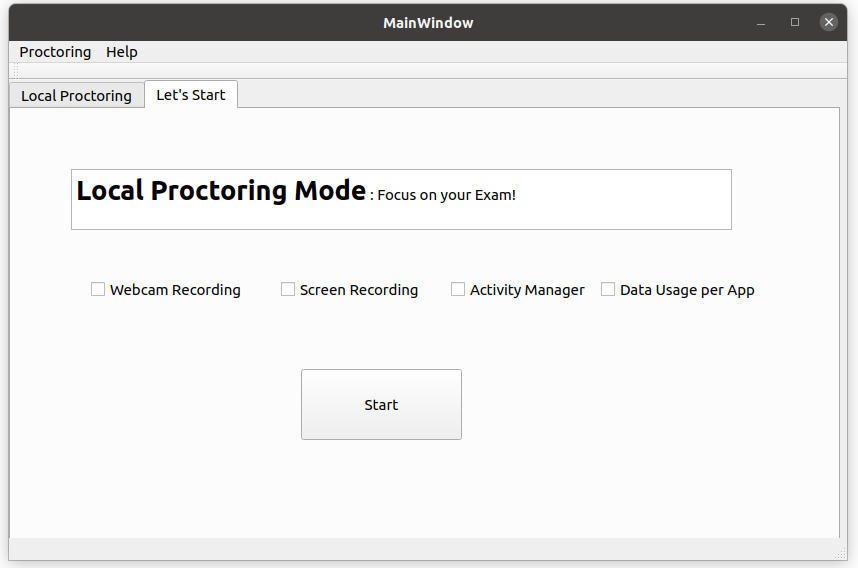
\includegraphics[scale=0.5]{LetsStart.png}    
\end{center}

\begin{enumerate}
    \item Here there are four check boxes named according to the functionalities they will provide, namely:
    \begin{enumerate}
        \item Webcam Recording
        \item Screen Recording
        \item Activity Manager
        \item Data usage per app
    \end{enumerate}
    \item Check on the required functionalities you want monitored during the proctoring.
\end{enumerate}

\subsubsection{functionality of each checkbox/function}
\begin{itemize}
    \item Webcam Recording: Accesses the webcam and records\\
    \textbf{Note: Internet loss triggered} - Webcam recording will only start if there is a loss in internet connectivity detected\\
    This assumes that you are already on some proctoring platform like ms teams initially and if there is a loss of internet connectivity then only webcam recording will start.\\
    \item Screen Recording: Records the entire computer screen\\
    \textbf{Note: Internet loss triggered} - Screen recording will only start if there is a loss in internet connectivity detected\\
    This assumes that you are already on some proctoring platform like ms teams initially and if there is a loss of internet connectivity then only webcam recording will start.\\
    \item Activity Manager: Monitors the activities related to which apps were used during the proctoring
    \item Data usage per app: monitors the data used by per app during the proctoring
\end{itemize}

After checking on the appropriate check boxes you can start the monitoring by clicking on "Start" button.\\
\begin{center}
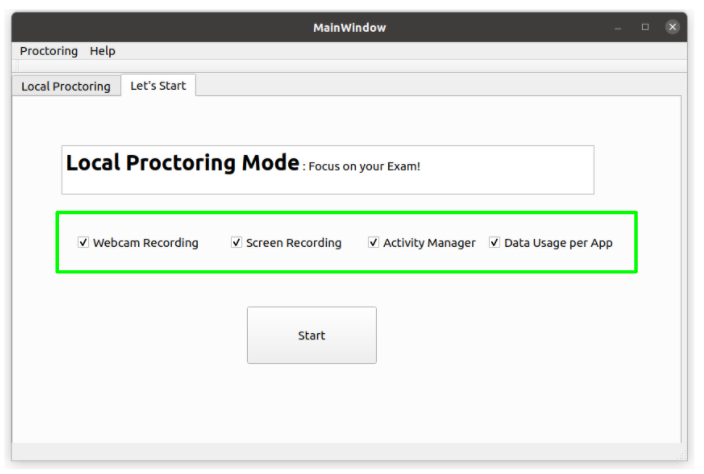
\includegraphics[scale=0.8]{checkbox.png}    
\end{center}
After clicking on start a new pop-up window will open\\
\begin{center}
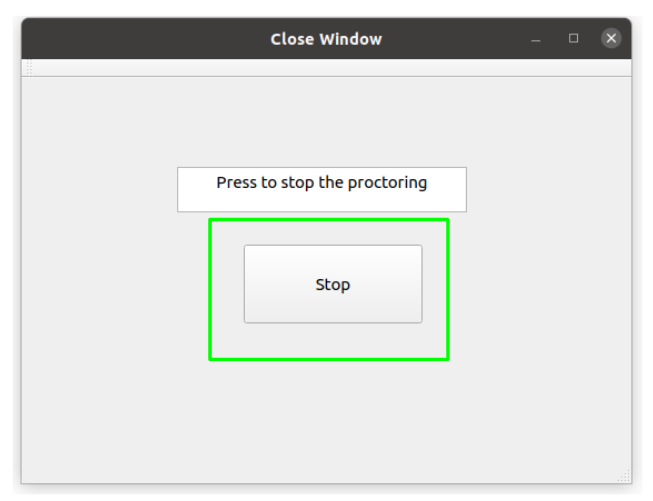
\includegraphics[scale=0.5]{close.png}    
\end{center}
Whenever you want to stop the proctoring/monitoring just click on the stop button.\\
This will close the application also.\\
All the corresponding outputs will be saved in the "Results" directory.\\


\subsection{Action bar - viewing the results}
\subsubsection{Proctoring}
This option will direct you to various log files and graphs generated by the software.
By clicking on this Menu Option you will get a drop-down with following options.\\
\begin{itemize}
    \item Results
    {
    \begin{itemize}
        \item Data Usage
        \item Activity Monitor
        \item Screen Recordings
        \item Video Recordings
    \end{itemize}}
    \item Graph
    \begin{itemize}
        \item Latest activity tracker
        \item Latest Data Usage
    \end{itemize}
\end{itemize}
\newpage
The Results section will take you the corresponding folder where log files and graphs are stored.\\

\begin{center}
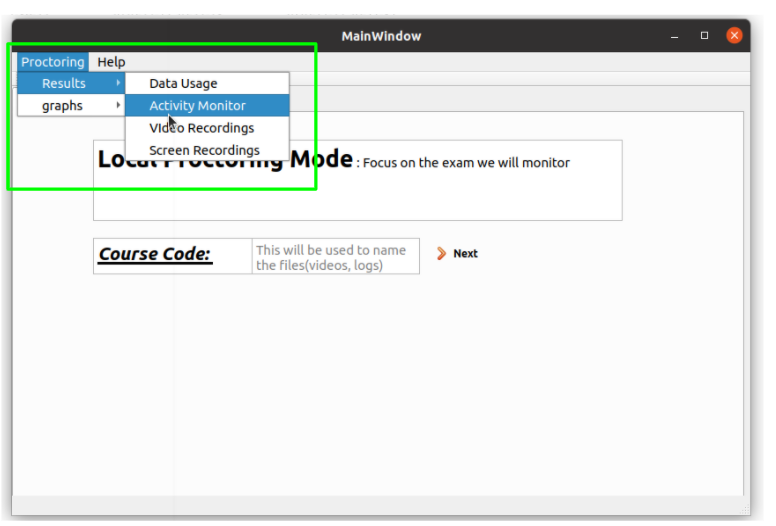
\includegraphics[scale=0.8]{menubar.png}    
\end{center}
\newpage
The Graph section will display the latest graph of the corresponding option you will select.\\\\
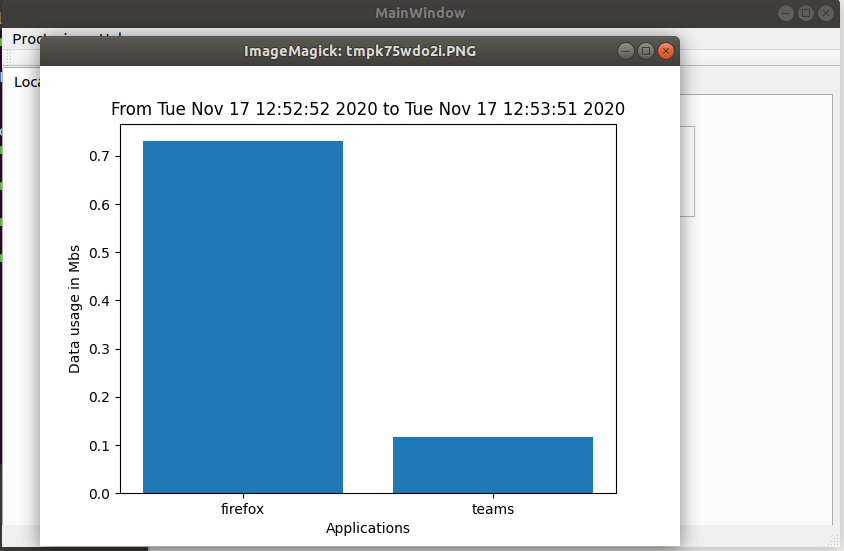
\includegraphics[scale=0.5]{Screenshot from 2020-11-17 14-13-03.png}
\newpage
\subsubsection{Help}
This option will display the open readme.txt to you which will direct you to the readme file.\\
\begin{center}
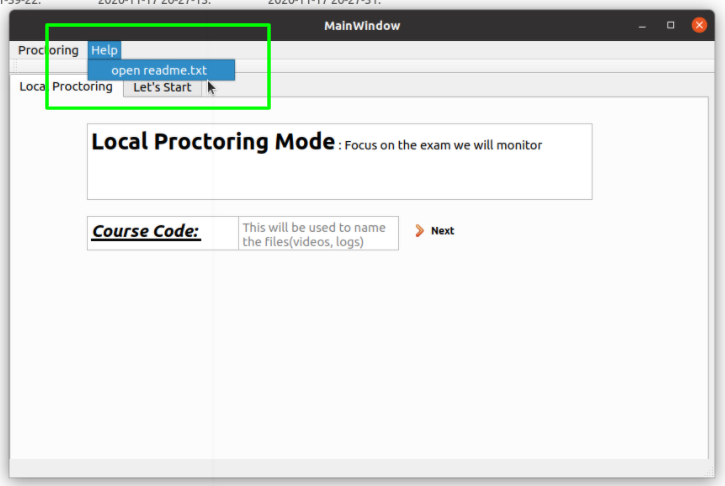
\includegraphics[scale=0.8]{Help.png}    
\end{center}
\subsection{Notification}
Two types of notification are issued to the user.
\begin{itemize}
    \item When Internet goes down.
    \item When Internet comes back.
\end{itemize}
\begin{center}
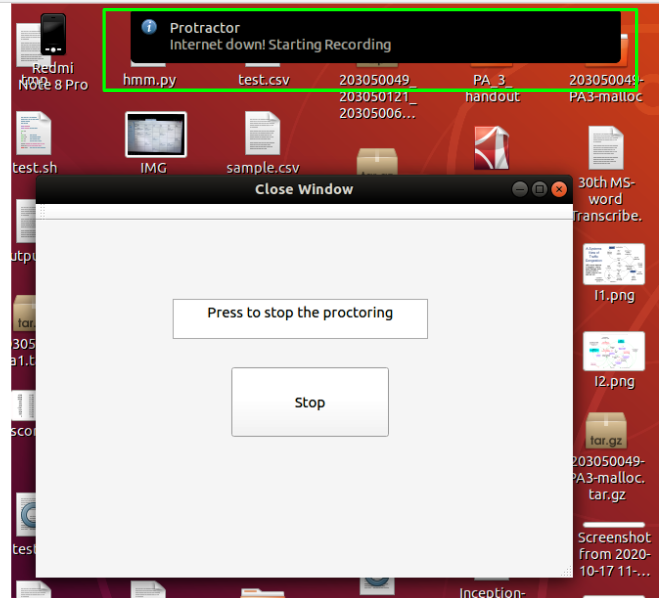
\includegraphics[scale=0.5]{InternetDown.png}    
\end{center}
\begin{center}
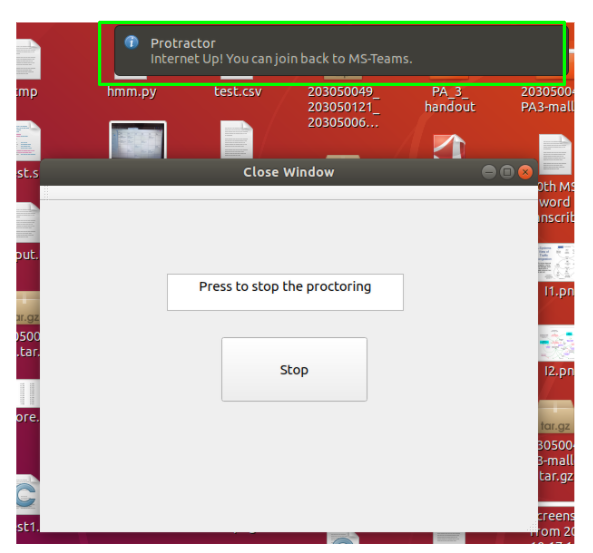
\includegraphics[scale=0.8]{InternetUp.png}    
\end{center}
\section{Usefulness}
The current scenario of online semester and online proctoring will most likely to continue in future and this local proctoring program is the first step in easing both students and invigilators burden by hassle free management due to loss of internet connection. The data generated in the form of log files, videos, time stamps, data usage, and activity usage can be used very efficiently for training of future AI based proctoring models. The initial runs of the program on the current video based proctoring through online channels were really useful. If used by the students or invigilators they will surely appreciate the usefulness of video recording and screen recording at the instant of internet loss and they can focus on the exam rather than focussing on the setup.
\section{Future Enhancements}
We would like to make the platform more robust with more functionalities. We would like to make the program support multiple platforms.\\
This Would be helpful in gathering data and making ai based proctoring systems

%----------------------------------------------------------------

\section{References}
\begin{enumerate}
    \item https://askubuntu.com/questions/779873/is-there-software-which-time-tracks-window-application-usage/780542#780542
    \item https://www.geeksforgeeks.org/bar-plot-in-matplotlib/
\end{enumerate}

\end{document}
